\documentclass{article}
\usepackage{graphicx}
\usepackage{amsmath}
\usepackage{amssymb}
\usepackage{amsthm}
\usepackage{mdframed}
\usepackage{xcolor}

\title{TEOREMA Y DEMOSTRACION}
\author{Juan Carlos Huanca Mamani}
\date{September 2024}


\definecolor{theoremcolor}{rgb}{0.8, 0.8, 1}
\definecolor{proofcolor}{rgb}{0.9, 1, 0.9}


\newmdenv[
  backgroundcolor=theoremcolor,
  linecolor=black,
  linewidth=2pt,
  roundcorner=10pt,
  innertopmargin=10pt,
  innerbottommargin=10pt,
  skipabove=10pt,
  skipbelow=10pt
]{theoremframe}


\newmdenv[
  backgroundcolor=proofcolor,
  linecolor=black,
  linewidth=2pt,
  roundcorner=10pt,
  innertopmargin=10pt,
  innerbottommargin=10pt,
  skipabove=10pt,
  skipbelow=10pt
]{proofframe}


\newtheorem{theorem}{Theorem}

\begin{document}
\maketitle
\begin{theoremframe}
\begin{theorem}
  (Dirichlet's Approximation Theorem) For any real number \(\alpha\) and any positive integer \(N\), there exist integers \(p\) and \(q\) with \(1 \leq q \leq N\) such that
  \[
  \left| \alpha - \frac{p}{q} \right| < \frac{1}{qN}.
  \]
\end{theorem}
\end{theoremframe}

\begin{proofframe}
\begin{proof}
  Consider the fractional parts \(\{n\alpha\}\) for \(n = 1, 2, \ldots, N+1\). There are \(N+1\) such fractional parts, but only \(N\) intervals of the form \(\left[ \frac{k}{N}, \frac{k+1}{N} \right)\) for \(k = 0, 1, \ldots, N-1\).

  By the pigeonhole principle, there must be two distinct integers \(m\) and \(n\) such that \(\{m\alpha\}\) and \(\{n\alpha\}\) lie in the same interval. Without loss of generality, assume \(m > n\). Then we have
  \[
  \left| \{m\alpha\} - \{n\alpha\} \right| < \frac{1}{N}.
  \]

  Let \(p = m - n\) and \(q = \left| \{m\alpha\} - \{n\alpha\} \right|\). Then \(1 \leq q \leq N\) and
  \[
  \left| \alpha - \frac{p}{q} \right| = \left| \alpha - \frac{m-n}{q} \right| < \frac{1}{qN}.
  \]

  This completes the proof.
\end{proof}
\end{proofframe}


\begin{center}
    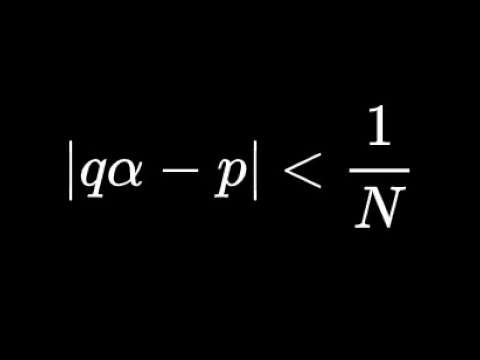
\includegraphics[scale=0.5]{teorema-de-aproximacion-de-dirichlet.jpg}
\end{center}


\begin{theoremframe}
\begin{theorem}
  (Generalization of Dirichlet's Theorem) Let \(\alpha_1, \alpha_2, \ldots, \alpha_n\) be real numbers. For any positive integer \(N\), there exist integers \(p_1, p_2, \ldots, p_n\) and \(q\) with \(1 \leq q \leq N\) such that
  \[
  \left| \alpha_i - \frac{p_i}{q} \right| < \frac{1}{qN} \quad \text{for all } i = 1, 2, \ldots, n.
  \]
\end{theorem}
\end{theoremframe}


\begin{proofframe}
\begin{proof}
  Consider the points \((\{n\alpha_1\}, \{n\alpha_2\}, \ldots, \{n\alpha_n\})\) for \(n = 1, 2, \ldots, N+1\) in the unit cube \([0, 1)^n\). There are \(N+1\) such points, but only \(N^n\) subcubes of side length \(\frac{1}{N}\).

  By the pigeonhole principle, there must be two distinct integers \(m\) and \(n\) such that the points \((\{m\alpha_1\}, \{m\alpha_2\}, \ldots, \{m\alpha_n\})\) and \((\{n\alpha_1\}, \{n\alpha_2\}, \ldots, \{n\alpha_n\})\) lie in the same subcube. Without loss of generality, assume \(m > n\). Then we have
  \[
  \left| \{m\alpha_i\} - \{n\alpha_i\} \right| < \frac{1}{N} \quad \text{for all } i = 1, 2, \ldots, n.
  \]

  Let \(p_i = m - n\) and \(q = \left| \{m\alpha_i\} - \{n\alpha_i\} \right|\). Then \(1 \leq q \leq N\) and
  \[
  \left| \alpha_i - \frac{p_i}{q} \right| < \frac{1}{qN} \quad \text{for all } i = 1, 2, \ldots, n.
  \]

  This completes the proof.
\end{proof}
\end{proofframe}


\end{document}
